\item \textbf{{[}YIJC/PRELIM/9569/2021/P2/Q2{]} }

Every user is required to carry a tracing token inside an indoor sports
facility so that the sensing device system can detect the token to
read the position of the users and their temperature. The data is
stored as records in the file \texttt{POSRECORDS.txt}, with the following
entries separated by commas: 
\begin{itemize}
\item the tag number (\texttt{INTEGER}) of the tracing token which could
be used to identify the user 
\item the temperature (\texttt{FLOAT}) of the user measured in degree Celsius 
\item the location $(x,y)$\texttt{ (FLOAT,FLOAT)} of the user which consists
of the perpendicular \texttt{x-} and \texttt{y-}distances, measured
in metres, from the walls A and B respectively 
\end{itemize}
The diagram below shows two locations $(x_{1},y_{1})$ and $(x_{2},y_{2})$: 
\noindent \begin{center}
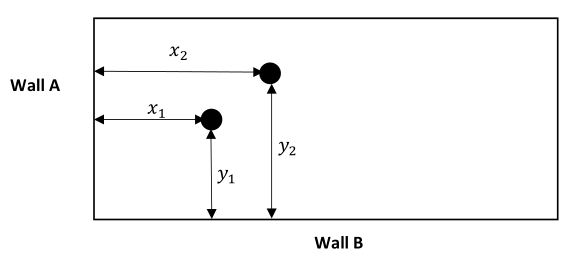
\includegraphics[scale=0.5]{C:/Users/Admin/Desktop/Github/question_bank/LyX/static/img/9569-YIJC-2021-P2-Q2}
\par\end{center}

The distance between two locations can be calculated using the formula: 

\[
\text{Distance}=\sqrt{(x_{2}-x_{1})^{2}+(y_{2}-y_{1})^{2}}
\]


\subsubsection*{Task 2.1 }

Create an empty array \texttt{all\_records} of size 20 and paste the
data from the text file \texttt{POSRECORDS.txt} into your program
code. 

Write program code for the function \texttt{distance(user1,user2)}
that takes in two records and returns the distance between the two
users in metres, correct to 2 decimal places. \hfill{} {[}3{]}

For safety reasons during the Covid-19 pandemic, two users are considered
to be in close proximity if the distance between them is less than
1.5 m apart. 

\subsubsection*{Task 2.2 }

Write program code for the function \texttt{analyse(user1)} that iterates
through all the records in the array \texttt{all\_records}, calculates
the distances between \texttt{user1} and all other users in the array,
and returns a list of tag numbers of the users who are in close proximity
to \texttt{user1}. \hfill{} {[}5{]}

Under the Safe Management Measures, people with a temperature of more
than 37.5 degree Celsius will be flagged out as RED cases and the
people who are in close proximity to these RED cases will be flagged
out as YELLOW cases. The facility manager needs to submit both lists
to the authority daily for follow-up actions. 

\subsubsection*{Task 2.3 }

Write program code for the function \texttt{red\_list(all\_records)}
that iterates through all the records in the array \texttt{all\_records}
and returns a list of tag numbers belonging to the RED cases. \hfill{}
{[}2{]}

\subsubsection*{Task 2.4 }

Write program code for the function \texttt{yellow\_list(red\_cases,all\_records)}
that iterates through all the records in the array \texttt{all\_records}
to check for people who were in close proximity to any of the RED
cases. The function returns a list of tag numbers belonging to the
YELLOW cases. 

Those people flagged out as RED cases in \textbf{Task 2.3} should
not appear in the list of YELLOW cases even though they may be in
close proximity to another RED case. 

You may use the functions written in Task 2.1 and Task 2.2 for the
program code in this task. \hfill{} {[}5{]}